% Project n. 3 ITY
% Jan Jakub Kubik (xkubik32)
% VUT FIT 2.4.2017

\documentclass[a4paper, 11pt, times]{article}

% ------------------------------------
% Required packages and basic setting
% ------------------------------------
\usepackage[left=2cm, top=3cm, text={17cm, 24cm}]{geometry}
\usepackage[utf8]{inputenc}
\usepackage[czech]{babel}
\usepackage{times}
\usepackage{mathptmx}
\usepackage{multirow}
\usepackage{graphicx}
\usepackage[ruled,czech,procnumbered]{algorithm2e}
\usepackage{algorithmic}
\usepackage{pdflscape}


% -----------
% Title page
% -----------
\begin{document}
\begin{center}
  \Huge\textsc{Vysoké učení technické v~Brně} \\
      \huge\textsc{Fakulta infrmačních technologií}\\
  \vspace{\stretch{0.382}}
  \huge Typografie a publikování \---\ 3.projekt\\
  \Huge{Tabulky a obrázky}
  \vspace{\stretch{0.618}}
\end{center}

{\LARGE \today \hfill Ján Jakub Kubík}
\thispagestyle{empty}
\newpage


% -------
% Page 1
% -------
\clearpage
\setcounter{page}{1}


% ----------
% Section 1
% ----------
\section{Úvodní strana}
Název práce umístněte do zlatého řezu a nezapomeňte
uvést dnešní datum a vaše jméno a příjmení


% ----------
% Section 2
% ----------
\section{Tabulky}
Pro sázení tabulek můžeme použít buď prostředí \texttt{tabbing} nebo prostředí \texttt{tabular}.


% Subsection 2.1
\subsection{Prostředí \texttt{tabbing}  }
Při použití \texttt{tabbing} vypadá tabulka následovně:


% Table 1 
\begin{tabbing}
  \textbf{Ovoce} \hspace{16mm}\= \textbf{Cena} \quad  \= \textbf{Mnozstvi}  \\
       Jablka \> 25,90 \> 3 kg \\
       Hrusky \> 27,40 \> 2,5 kg \\
       Vodni melouny \> 25,-- \> 1 kus
\end{tabbing}
Toto prostředí se dá také použít pro sázení algoritmů, ovšem vhodnější je použít
prostředí \texttt{algorithm}| nebo \texttt{algorithm2e}  (viz sekce 3).


% Subsection 2.2 
\subsection{Prostředí \texttt{tabular} }
Další možností, jak vytvořit tabulku, je použít prostředí \texttt{tabular}. Tabulky pak
budou vypadat takto\footnotemark[1]:
\begin{table}[h]
\centering
 \catcode`\-=12
\begin{tabular}{|c|c|c|}
\hline
 & \multicolumn{2}{c|}{\textbf{Cena}} \\ \cline{2-3}
\textbf{Měna} & \textbf{nákup}  & \textbf{prodej} \\ \hline
EUR               & 27,02           & 27,20  \\
GPB               & 31,08           & 31,80  \\
USD               & 25,15           & 25,51  \\
\hline
\end{tabular}
\caption{Tabulka kurzů k dnešnímu dni}
\label{tab:small_table}
\end{table}


% Big table
\begin{table}[h]
\begin{center}
\catcode`\-=12
  

  % Subtable 1
  \begin{tabular}{|c|c|}
    \hline
    $A$           &     $ \neg A $ \\ \hline
    \textbf{P}    &     $ N $      \\ \hline
    \textbf{O}    &     O          \\ \hline
    \textbf{X}    &     X          \\ \hline
    \textbf{N}    &     P          \\ \hline
  \end{tabular}


  % Subtable 2
  \begin{tabular}{ |c|c|c|c|c|c| }
    \hline
    \multicolumn{2}{|c}{\multirow{2}{*}{$A \land B$ }} & \multicolumn{4}{|c|}{$B$} \\ \cline{3-6}
    \multicolumn{2}{|c|}{} &  \textbf{P}  & \textbf{O}  & \textbf{X}  & \textbf{N} \\ \hline
    \multirow{4}{*}{$A$} & \textbf{P} & P & O & X & N \\ \cline{2-6}
    &                      \textbf{O} & O & O & N & N \\ \cline{2-6}
    &                      \textbf{X} & X & N & X & N \\ \cline{2-6}
    &                      \textbf{N} & N & N & N & N \\ \hline
  \end{tabular}


  % Subtable 3
  \begin{tabular}{ |c|c|c|c|c|c| }
  \hline
  \multicolumn{2}{|c}{\multirow{2}{*}{$A \lor B$ }} & \multicolumn{4}{|c|}{$B$} \\ \cline{3-6}
    \multicolumn{2}{|c|}{} &   \textbf{P}  & \textbf{O}  & \textbf{X}  & \textbf{N} \\ \hline
    \multirow{4}{*}{$A$} & \textbf{P} & P & P & P & P \\ \cline{2-6}
    &                      \textbf{O} & P & O & P & O \\ \cline{2-6}
    &                      \textbf{X} & P & P & X & X \\ \cline{2-6}
    &                      \textbf{N} & P & O & X & N \\ \hline
  \end{tabular}


  % Subtable 4
  \begin{tabular}{ |c|c|c|c|c|c| }
  \hline
  \multicolumn{2}{|c}{\multirow{2}{*}{$A \lor B$ }} & \multicolumn{4}{|c|}{$B$} \\ \cline{3-6}
    \multicolumn{2}{|c|}{} &   \textbf{P}  & \textbf{O}  & \textbf{X}  & \textbf{N} \\ \hline
    \multirow{4}{*}{$A$} & \textbf{P} & P & O & X & N \\ \cline{2-6}
    &                      \textbf{O} & P & O & P & O \\ \cline{2-6}
    &                      \textbf{X} & P & P & X & X \\ \cline{2-6}
    &                      \textbf{N} & P & P & P & P \\ \hline
  \end{tabular}
\caption{Protože Kleeneho trojhodnotová logika už je \uv{zastaralá}, uvádime
          si zde příklad čtyřhodnotové logiky}
\label{tab:big_table}
\end{center}
\end{table} % end of Big table

\footnotetext[1]{Kdyby byl problem s \texttt{cline}, zkuste se podvat třeba sem:
\textup{http://www.abclinuxu.cz/tex/poradna/show/325037}}

\newpage


% -------
% Page 2
% ------


% ----------
% Section 3
% ----------
\section{Algoritmy}
Pokud budeme chtít vysázet algoritmus, můžeme použít prostředí \texttt{algorithm}\footnotemark[2] \ nebo \texttt{algorithm2e}\footnotemark[3].
Příklad použití prostředí \texttt{algorithm2e} viz Algoritmus 1.\\


% Algorithm implementation
\begin{algorithm}[H]
	\caption{\textsc{FastSLAM}}
  \label{alg:algoritmus}
	\SetKwInput{Input}{Input}
	\SetKwInOut{Output}{Output}

	\Input{$(X_{t-1},u_t,z_t)$}
	\Output{$X_t$}

	\BlankLine
	\Indp\Indp
	 \begin{algorithmic}[1]
		\STATE $ \overline{X_t}=X_t=0$
		\FOR{$k = 1$ to $M$}
		    \STATE ${x_t}^{[k]}=sample\_motion\_model(u_t,x_{t-1}^{[k]})$
		    \STATE ${\omega_t}^{[k]}=measurement\_model(z_t,x_t^{[k]},m_{t-1})$
		    \STATE ${m_t}^{[k]}=updated\_occupancy\_grid(z_t,x_{t}^{[k]},m_{t-1}^{[k]})$
		    \STATE $\overline{X_t}=X_t +\langle x_x^{[m]}, \omega_t^{[m]}\rangle$
		\ENDFOR
		\FOR{$k = 1$ to $M$}
		    \STATE draw $i$ with probability $ \approx \omega_t^{[i]}$
		    \STATE add $\langle x_x^{[k]},m_t^{[k]}\rangle $ to $X_t$
		\ENDFOR
		\RETURN $X_t$
\end{algorithmic}
\end{algorithm}

\footnotetext[2]{Pro nápovědu, jak zacházet s prostředím \texttt{algorithm}, múžeme zkusit tuhle stránku:\\
\textup{http://ftp.cstug.cz/pub/tex/CTAN/macros/latex/contrib/algorithms/algorithms.pdf.}}
\footnotetext[3]{Pro \texttt{algorithm2e} zase tuhle:
\textup{http://ftp.cstug.cz/pub/tex/CTAN/macros/latex/contrib/algorithm2e/algorithm2e.pdf.}}


% ----------
% Section 4
% ----------
\section{Obrázky}

Do našich článků múžeme samozřejmě vkládat obrázky. Pokud je obrázkem fotografie,
múžeme klidně použít bitmapový soubor. Pokud by to ale mělo být nějaké schéma nebo
něco podobného, je dobrým zvykem takovýto obrázek vytvořit vektorově.


% Image 
\begin{figure}[h]
\begin{center}
    \scalebox{0.45}{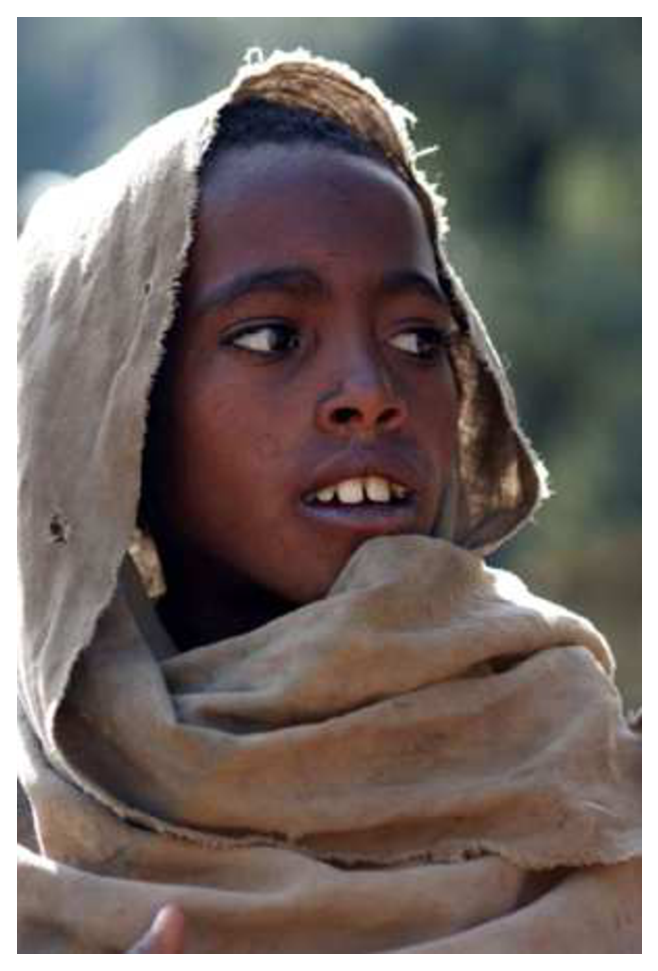
\includegraphics{etiopan.eps}
    \reflectbox{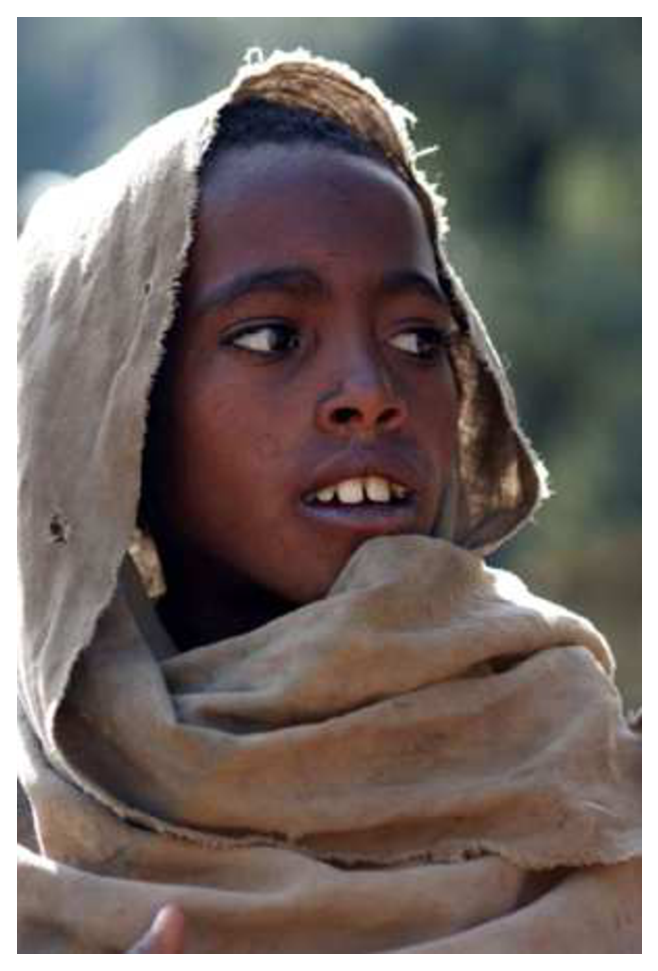
\includegraphics{etiopan.eps}} }
\caption{Malý Etiopánek a jeho bratříček}
\label{fig:africa}
\end{center}
\end{figure}


% -------
% Page 3
% -------
Rozdíl mezi vektorovým\ .\ .\ .
\begin{figure}[h]
\begin{center}
\scalebox{0.45}{
\includegraphics{oniisan.eps}}
\caption{Vekotový obrázek}
\label{fig:vector}
\end{center}
\end{figure}

.\ .\ . a bitmapovým obrázkem
\begin{figure}[h]
\begin{center}
\scalebox{0.65}{
\includegraphics{oniisan2.eps} }
\caption{Bitmapový obrázek}
\label{fig:bitmap}
\end{center}
\end{figure}

\noindent{se projeví například při zvětšení.}

Odkazy (nejen ty) na obrázky \ref{fig:africa}, \ref{fig:vector} a \ref{fig:bitmap}, na
tabulky \ref{tab:small_table} a \ref{tab:big_table} a také na algoritmus \ref{alg:algoritmus} jsou udělány pomocí
křížových odkazů. Pak je ovšem potřeba zdrojový soubor přeložit dvakrát. \\
Vektorové obrázky lze vytvořit i přímo v \LaTeX u, například pomocí prostředí
\texttt{picture}.


% -------
% Page 4
% -------
\begin{landscape}
\begin{figure}[h]
\centering
\setlength{\unitlength}{1mm}
\begin{picture}(200,100)
\put(0,0){\linethickness{1pt}\framebox(200,100){}}
\put(170,80){\circle{70}}


% Upper part
\linethickness{0.5mm}
\put(68,56){\line(1,0){55}}
\put(123,46){\line(0,0){10}}
\put(43	,46){\line(1,0){139}}
\put(123,48){\line(1,0){49}}
\put(172,46){\line(0,0){2}}
\put(24,15){\line(0,0){36}}
\put(24,51){\line(1,0){44}}
\put(68,46){\line(0,0){10}}
\put(182,40){\line(0,0){6}}
\put(43,40){\line(0,0){6}}
\put(43	,40){\line(1,0){139}}
\put(43	,40){\line(1,-1){11}}


% Bottom part
\put(182,15){\line(0,0){9}}
\put(86,24){\line(1,0){96}}
\put(179,24){\line(0,0){14}}
\put(73,38){\line(1,0){106}}
\put(35	,15){\line(0,0){14}}
\put(35	,29){\line(1,0){36}}
\put(71	,29){\line(3,-1){40}}
\put(73,29){\line(0,0){9}}


% Biggest line
\linethickness{1.5mm}
\put(4,15){\line(1,0){190}}

\end{picture}
\caption{Vektorový obrázek}
\end{figure}
\end{landscape}

\end {document}
